\documentclass[11pt,letter, swedish, english
]{article}
\pdfoutput=1

\usepackage{../custom_as}
\usepackage[makeroom
]{cancel}
\graphicspath{{figures/}}

\swapcommands{\Delta}{\varDelta}
\swapcommands{\Omega}{\varOmega}

%%Drar in tabell och figurtexter
\usepackage[margin=10 pt]{caption}
%%För att lägga in 'att göra'-noteringar i texten
\usepackage{todonotes} %\todo{...}

%%För att själv bestämma marginalerna. 
\usepackage[
%            top    = 2.5cm,
%            bottom = 3cm,
%            left   = 3cm, right  = 3cm
]{geometry}

%%För att ändra hur rubrikerna ska formateras


\renewcommand{\thefootnote}{\fnsymbol{footnote}}

\newcommand{\Tc}{\ensuremath{T_{\text{c}}}}
\newcommand{\eF}{\ensuremath{\epsilon_{\text{F}}}}
\newcommand{\wD}{\ensuremath{\omega_{\text{D}}}}

%\usepackage{tikz}

\begin{document}

%\tikzstyle{every picture}+=[remember picture]
%\tikzstyle{na} = [shape=rectangle,inner sep=0pt,text depth=0pt]



%%%%%%%%%%%%%%%%% vvv Inbyggd titelsida vvv %%%%%%%%%%%%%%%%%

\title{Statistical Physics 2 -- PHYS\,705 \\
Assignment 1}
\author{Andréas Sundström}
\date{\today}

\maketitle

%%%%%%%%%%%%%%%%% ^^^ Inbyggd titelsida ^^^ %%%%%%%%%%%%%%%%%

\section{Mean field magnetic susceptibility}
\renewcommand{\thesubsection}{\arabic{section} (\roman{subsection})}

In this problem, we will study the magnetic susceptibility, $\chi$, in
view of the MFT approach to the Ising model. We will look at the
asymptotic behaviour of $\chi$ for $T\to0^+$ and $T\to\Tc$.

We begin from the MF equation
\begin{equation}\label{eq:1_MFE}
M=\tanh(\frac{MJ + B}{T}),
\end{equation}
and the definition of susceptibility
\begin{equation}\label{eq:1_chi}
\chi:=\eval{\dv{M}{B}}_{B=0}.
\end{equation}

By applying \eqref{eq:1_chi} to \eqref{eq:1_MFE}, we get
\begin{equation}
\chi=\frac{1}{\cosh^2(MJ/T)}\, 
\qty(\frac{J}{T}\chi+\frac{1}{T}),
\end{equation}
or in other words
\begin{equation}\label{eq:1_chi_exact}
\chi=\frac{1}{T\cosh^2(M\Tc/T)-\Tc}.
\end{equation}
In the last step we also used the fact that $\Tc=J$ using the MFT approach.

\subsection{Zero temperature limit}
As $T\to0^+$, the leading order behaviour of the hyperbolic cosine is
\begin{equation}
\cosh^2\qty(\frac{M\Tc}{T})\sim \frac{1}{4}\exp(2\frac{\abs{M}\Tc}{T}).
\end{equation}
This exponential growth will dominate over the factor $T$ in
front and the constant $-\Tc$ in the denominator. And \eqref{eq:1_MFE}
also shows us that $M\to\pm1$ as $T\to0^+$. 

The asymptotic behaviour of \eqref{eq:1_chi_exact} will be 
\begin{equation}
\chi\sim \frac{4}{T}\exp(-2\frac{\Tc}{T})
\qcomma \text{as}\ T\to0.
\end{equation}
And to be clear, this asymptotic behaviour results in $\chi(T)\to0$ as
$T\to0$. 


\subsection{Critical temperature limit}
We begin with aproaching the limit from below, $T<\Tc$. We do still
evaluate the derivative for $\chi$ at $B=0$, so the MFT value for $M$
can be used:
\begin{equation}
M=\sqrt{3}\frac{T}{\Tc}\sqrt{-t}.
\end{equation}
Plugging this into the exact expression \eqref{eq:1_chi_exact} and
Taylor expanding the hyperbolic cosine gives
\begin{equation}
\begin{aligned}
\chi(T\to\Tc^-)\sim&\frac{1}{T\qty[1+3(T/\Tc)^2(\Tc-T)/\Tc]-\Tc}\\
=&\frac{1}{T-3(T/\Tc)^3(T-\Tc) -\Tc}\\
=&\frac{1}{T-\Tc}\times\frac{1}{1-3(T/\Tc)^3}\\
\sim&\frac{1}{2}\times\frac{1}{\Tc-T}=\frac{1}{2\Tc}|t|^{-1}.
\end{aligned}
\end{equation}
If we approach the limit from the other end, we know that $M=0$. So
\eqref{eq:1_chi_exact} is just
\begin{equation}
\chi(T\to\Tc^+)=\frac{1}{T-\Tc}=\frac{1}{\Tc} |t|^{-1}.
\end{equation}

To conclude this part of the problem we note that in both cases, we
can write
\begin{equation}
\chi=C_\pm |t|^{-\gamma},
\end{equation}
where $\gamma=1$ and $C_+/C_-=2$.



\section{Phase transitions in Landau theory}
\renewcommand{\thesubsection}{\arabic{section} (\alph{subsection})}
\renewcommand{\thesubsubsection}{\arabic{section} (\alph{subsection},\,\roman{subsubsection})}

Here, we will use the Landau free energy
\begin{equation}\label{eq:2_F(M)}
F=-bM+tM^2+uM^4+M^6,
\end{equation}
where $b=B/T$, $t=(T-\Tc)/\Tc$ and $u$ is some coefiicient with no
restrictions. 

\subsection{Generic forms of $F$}
There will be, depending on how precise you want to be, around four
different generic forms of $F$, and they occur at
\begin{enumerate}[label=\Roman*.]
\item $t\ge0$, $u\ge0$ \\
Here, it's obvious that all we can get is a single minimum at $M=0$.
\item $t<0$, $u$ any value; or $t=0$, $u<0$\\
For $t<0$, the initial behaviour around $M=0$ is to drop down, but at
large $|M|$ we still get $F\to+\infty$. So we must have two minima at
$M\neq0$, and a local maximum at $M=0$. The same is true for $t=0$ and
$u<0$. 
\item $0<t<u^2/4$, $u<0$\footnotemark{}\addtocounter{footnote}{-1}\\
Here, we initially get a growing $F$, near $M=0$, but the effects of a
negative enough $u$ will then come into play and force down $F(m)$ to
two minima at $M\neq0$ which are stronger than the one at $M=0$.
\item $t>u^2/4$, $u<0$\footnotemark{}\\
In this case, there might not even be two minima at $M\neq0$, but if
they excist they are weaker than the one at $M=0$.
\end{enumerate}
These four cases encompass all of the $u{-}T$ plane. The generic forms
of $F(M)$ can be seen in \figref{fig:2a}.

\footnotetext{The difference between these two cases will be
  further elaborated on in part (b) of this problem.}

\begin{figure}
\centering
% GNUPLOT: LaTeX picture with Postscript
\begingroup
  \makeatletter
  \providecommand\color[2][]{%
    \GenericError{(gnuplot) \space\space\space\@spaces}{%
      Package color not loaded in conjunction with
      terminal option `colourtext'%
    }{See the gnuplot documentation for explanation.%
    }{Either use 'blacktext' in gnuplot or load the package
      color.sty in LaTeX.}%
    \renewcommand\color[2][]{}%
  }%
  \providecommand\includegraphics[2][]{%
    \GenericError{(gnuplot) \space\space\space\@spaces}{%
      Package graphicx or graphics not loaded%
    }{See the gnuplot documentation for explanation.%
    }{The gnuplot epslatex terminal needs graphicx.sty or graphics.sty.}%
    \renewcommand\includegraphics[2][]{}%
  }%
  \providecommand\rotatebox[2]{#2}%
  \@ifundefined{ifGPcolor}{%
    \newif\ifGPcolor
    \GPcolortrue
  }{}%
  \@ifundefined{ifGPblacktext}{%
    \newif\ifGPblacktext
    \GPblacktexttrue
  }{}%
  % define a \g@addto@macro without @ in the name:
  \let\gplgaddtomacro\g@addto@macro
  % define empty templates for all commands taking text:
  \gdef\gplbacktext{}%
  \gdef\gplfronttext{}%
  \makeatother
  \ifGPblacktext
    % no textcolor at all
    \def\colorrgb#1{}%
    \def\colorgray#1{}%
  \else
    % gray or color?
    \ifGPcolor
      \def\colorrgb#1{\color[rgb]{#1}}%
      \def\colorgray#1{\color[gray]{#1}}%
      \expandafter\def\csname LTw\endcsname{\color{white}}%
      \expandafter\def\csname LTb\endcsname{\color{black}}%
      \expandafter\def\csname LTa\endcsname{\color{black}}%
      \expandafter\def\csname LT0\endcsname{\color[rgb]{1,0,0}}%
      \expandafter\def\csname LT1\endcsname{\color[rgb]{0,1,0}}%
      \expandafter\def\csname LT2\endcsname{\color[rgb]{0,0,1}}%
      \expandafter\def\csname LT3\endcsname{\color[rgb]{1,0,1}}%
      \expandafter\def\csname LT4\endcsname{\color[rgb]{0,1,1}}%
      \expandafter\def\csname LT5\endcsname{\color[rgb]{1,1,0}}%
      \expandafter\def\csname LT6\endcsname{\color[rgb]{0,0,0}}%
      \expandafter\def\csname LT7\endcsname{\color[rgb]{1,0.3,0}}%
      \expandafter\def\csname LT8\endcsname{\color[rgb]{0.5,0.5,0.5}}%
    \else
      % gray
      \def\colorrgb#1{\color{black}}%
      \def\colorgray#1{\color[gray]{#1}}%
      \expandafter\def\csname LTw\endcsname{\color{white}}%
      \expandafter\def\csname LTb\endcsname{\color{black}}%
      \expandafter\def\csname LTa\endcsname{\color{black}}%
      \expandafter\def\csname LT0\endcsname{\color{black}}%
      \expandafter\def\csname LT1\endcsname{\color{black}}%
      \expandafter\def\csname LT2\endcsname{\color{black}}%
      \expandafter\def\csname LT3\endcsname{\color{black}}%
      \expandafter\def\csname LT4\endcsname{\color{black}}%
      \expandafter\def\csname LT5\endcsname{\color{black}}%
      \expandafter\def\csname LT6\endcsname{\color{black}}%
      \expandafter\def\csname LT7\endcsname{\color{black}}%
      \expandafter\def\csname LT8\endcsname{\color{black}}%
    \fi
  \fi
  \setlength{\unitlength}{0.0500bp}%
  \begin{picture}(9070.00,8502.00)%
    \gplgaddtomacro\gplbacktext{%
      \csname LTb\endcsname%
      \put(192,6220){\rotatebox{-270}{\makebox(0,0){\strut{}$F(M, t, u)$}}}%
      \put(2267,4419){\makebox(0,0){\strut{}$M$}}%
      \put(2267,8141){\makebox(0,0){\strut{}I. $t\ge0$, $u\ge0$}}%
    }%
    \gplgaddtomacro\gplfronttext{%
    }%
    \gplgaddtomacro\gplbacktext{%
      \csname LTb\endcsname%
      \put(4727,6220){\rotatebox{-270}{\makebox(0,0){\strut{}$F(M, t, u)$}}}%
      \put(6802,4419){\makebox(0,0){\strut{}$M$}}%
      \put(6802,8141){\makebox(0,0){\strut{}II. $t<0$, $u$ any value; or $t=0$, $u<0$}}%
    }%
    \gplgaddtomacro\gplfronttext{%
    }%
    \gplgaddtomacro\gplbacktext{%
      \csname LTb\endcsname%
      \put(192,1969){\rotatebox{-270}{\makebox(0,0){\strut{}$F(M, t, u)$}}}%
      \put(2267,168){\makebox(0,0){\strut{}$M$}}%
      \put(2267,3891){\makebox(0,0){\strut{}III. $0<t<u^2/4$, $u<0$}}%
    }%
    \gplgaddtomacro\gplfronttext{%
    }%
    \gplgaddtomacro\gplbacktext{%
      \csname LTb\endcsname%
      \put(4727,1969){\rotatebox{-270}{\makebox(0,0){\strut{}$F(M, t, u)$}}}%
      \put(6802,168){\makebox(0,0){\strut{}$M$}}%
      \put(6802,3891){\makebox(0,0){\strut{}IV. $t>u^2/4$, $u<0$}}%
    }%
    \gplgaddtomacro\gplfronttext{%
      \csname LTb\endcsname%
      \put(7854,891){\makebox(0,0)[r]{\strut{}$t>u^2/4$, but not by much}}%
      \csname LTb\endcsname%
      \put(7854,651){\makebox(0,0)[r]{\strut{}$t\gg u^2/4$}}%
    }%
    \gplbacktext
    \put(0,0){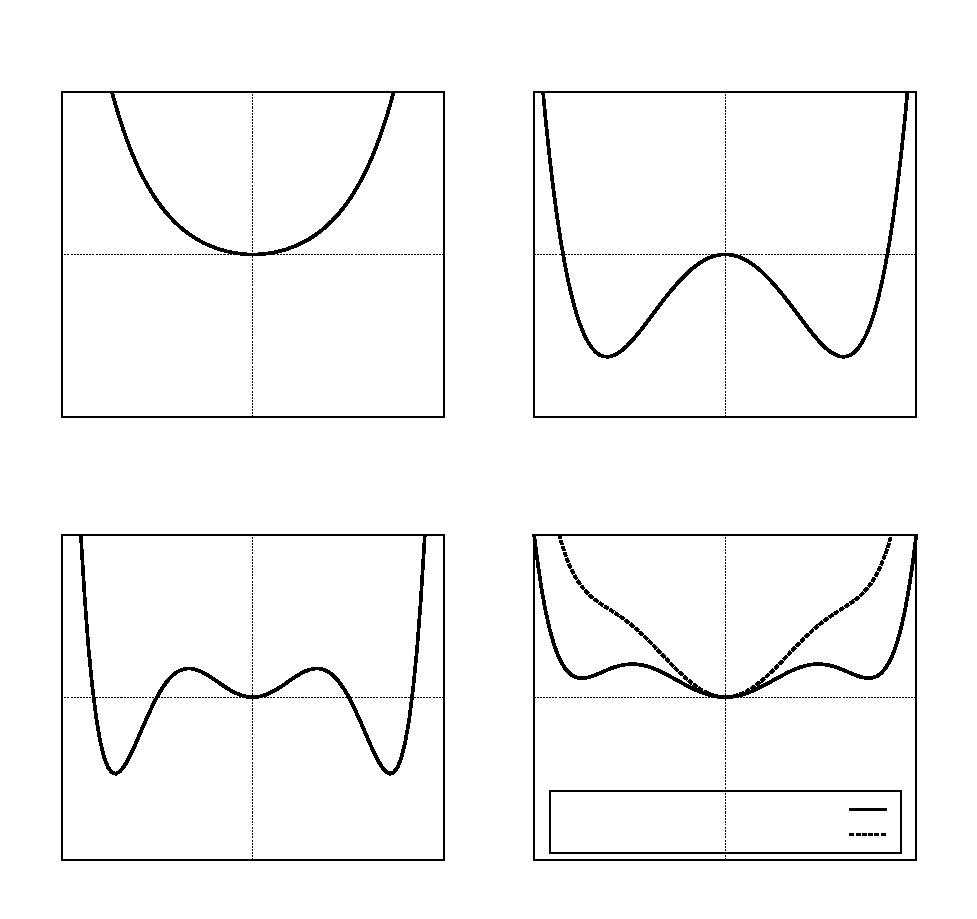
\includegraphics{generic_forms}}%
    \gplfronttext
  \end{picture}%
\endgroup

\caption{The four (or five) different generic forms of $F(M)$, as
  given by \eqref{eq:2_F(M)}. }
\label{fig:2a}
\end{figure}

\subsection{First order transition, when $u<0$}
As illustrated in the difference between case III and IV, we see that
when $u<0$ it is indeed possible to get a scenario when the global
minimum of $F(M)$ jumps from $M=0$ to $\pm M_0\neq0$. The transition
occurs when the equation 
\begin{equation}
tM^2+uM^4+M^6=M^2(t+uM^2+M^4)=0
\end{equation}
goes from only one real solution to three/five. This is because we
know that the minimum at $M=0$ gives $F(M=0)=0$. So if we were to get
more solutions to this equation, that would mean that $F$ can assume
negative values. Ergo, there are some other minima which are stronger
than the one at $M=0$. 

We are therefore looking for when
\begin{equation}
t+uM^2+M^4=0
\end{equation}
starts having real solutions. These solutions are
\begin{equation}
M^2=\frac{-u\pm\sqrt{u^2-4t}}{2},
\end{equation}
and we see that this occurs only if $t\le u^2/4$. We are now in case
III, where the \emph{global} minima is away from $M=0$. But $M=0$ is
still however a \emph{local} minimum; this means that there is a
chance that the system will remain in $M=0$ all the way until $t=0$,
when we enter case II. In case II, $M=0$ is instead a local maximum so the
system will quickly find its way to one of the two minima with
non-zero $M$. 

% Note also that the temperature at which this sudden jump in
% magetization happens is at $t=u^2/4>0$. That is the phase
% transition occurs at a temerature above $\Tc$.


\subsection{The tri-critical point}

\subsubsection{Phase transitions}
From the analysis in the previous part of the problem, we know that
the line of the first order transition is at $t=u^2/4$. This is
however only valid for $u<0$, so the first order transition line ends
at $(t, u)=(0, 0)$; that is the tri-critical point.

The second order phase transition is on the $t=0$ line with
$u\ge0$. All of this is ilustrated in \figref{fig:2_phase}.

\begin{figure}\centering
\input{figures/phase_diagram.pdf_t}
\caption{A phase diagram showing the reagions where the different
  cases, from the previous figure, are located. Case I and IV are 
  uncondensed, whereas case II and III are condensed phases. There
  might be some hysterisis involved in case III. }
\label{fig:2_phase}
\end{figure}

\subsubsection{Critical exponents}
Here we're going to find the critical exponents as we approach the
tri-critical point along the $u=0$ line. 

Let's begin by $\beta$. For this we need to know
$M(t,B=0)\propto(-t)^\beta$. We just use \eqref{eq:2_F(M)} and
differentiate both sides, remembering that $u=b=0$:
\begin{equation}\label{eq:2ii_M}
2tM+6M^5=0\quad\Longrightarrow\quad
M=\qty(-\frac{1}{3}t)^{1/4}.
\end{equation}
So $\beta=1/4$.

Next is $\gamma$: $\chi=C_\pm|t|^{-\gamma}$. To get $\chi$ we need to
keep the term involving $b$ when we calculate $M$:
\begin{equation}\label{eq:2ii_gamma}
-b+2tM+6M^5=0.
\end{equation}
For $t>0$, we can assume that $M\ll1$ which means that the $M^5$ term
can be disregarded ($M^5\lll1$). This gives us $M=b/(2t)$ or
\begin{equation}
\chi(T\to\Tc^+)=\frac{1}{2t}.
\end{equation}
For $t<0$, we need a bit more work.
Assuming $b\ll t$, we can use perturbation theory and write
$M(b)=M_0+bM_1+\ldots$. By substituing this into \eqref{eq:2ii_gamma},
we get
\begin{equation}
\begin{aligned}
0=&-b+2t(M_0+bM_1)+6(M_0+bM_1)^5+\order{b^2}\\
=& \qty(M_0+6M_0^5)+b\qty(-1+2tM_1+30M_0^4M_1) +\order{b^2}.
\end{aligned}
\end{equation}
The unperturbed solution $M_0$ is just what we got in
\eqref{eq:2ii_M}, and since the above equation should hold for any
$b$ we have
\begin{equation}
\qty(-1+2tM_1+30M_0^4M_1)=0 \quad\Longrightarrow\quad
M_1=\frac{1}{2t+30M_0^4}=\frac{1}{8|t|}.
\end{equation}
So in this case we got $\gamma=1$, and $C_+/C_-=4$.

Next we can take $\alpha$:
$C_V=-T\dv*[2]{F}{T}=A_\pm|t|^{-\alpha}$. For $t>0$, we have $\dv{M}{T}=0$
meaning that $\dv[2]{F}{T}=0$. For $t<0$ however, we get $M$ as in
\eqref{eq:2ii_M} which results in
\begin{equation}
F(t<0, u=0, b=0)=t(-\frac{1}{3}t)^{1/2}+(-\frac{1}{3}t)^{3/2}
=-\frac{2}{3\sqrt{3}}(-t)^{3/2}.
\end{equation}
This, in turn, gives
\begin{equation}
C_V=-T\dv[2]{F}{(-t)}\qty(\dv{(-t)}{T})^2=\ldots
=\frac{T}{2\sqrt{3}\Tc}|t|^{-1/2}.
\end{equation}
So here we got $\alpha=1/2$, $A_-=1/(2\sqrt{3})$ and $A_+=0$.

And lastly we have $\delta$: $M(b,t=0)\propto b^{1/\delta}$. This time
we can again use \eqref{eq:2ii_gamma}, but with $t=0$, which gives
\begin{equation}
M=\qty(\frac{1}{6}b)^{1/5},
\end{equation}
or in other words $\delta=5$.



\section{1D Ising model}



\section{Ising model generalization}
The simple Ising model only has a symmetry between positiv and
negative $\varphi$, therefor the Landau free enregy $F$ is expressed in
terms of $\varphi^2$. If we however consider a model with rotational
symmery in $n$ dimansions, we should still express $F$ in terms of
something invariant under rotations. The simplest such object is
$\varphi_i\varphi_i=\vb*{\varphi}\vdot\vb*{\varphi}$. And the Landau
free energy, in its simplest form, can be written as
\begin{equation}
F(\varphi_i)=-\vb*{b}\vdot\vb*{\varphi}+t\vb*{\varphi}\vdot\vb*{\varphi}
+(\vb*{\varphi}\vdot\vb*{\varphi})^2.
\end{equation}
The units are also rescaled so that the coefficient in front of the
last term is $1$. 

As before, we see that (in the absence of $\vb*{b}$) the behaviour of
$F$ is very similar to the 1D version. For instance, at $t>0$ the
minimum of $F$ will occur at $\vb*{\varphi}\vdot\vb*{\varphi}=0$
meaning that $\ev{\varphi_i}=0$. Where as when $t<0$, we would get
some non-zero minimum where $|\vb*\varphi|=(-t/2)^{1/2}>0$ and
$\ev{\varphi_i}\neq0$ at least for some $i$'s. 

In the absence of a magnetic field, there is no perfered
direction. And yet, the system will fall into a $\vb*\varphi$ pointing
in some direction --- spontaneous symmetry-breaking. Apart from the 1D
case, the broken symmetry can however change continuously. The only
restriction on $\vb*\varphi$ is that its magnitue is some specific
value, other than that $\vb*\varphi$ is free to rotate in any
direction.

The critical exponents will be the same as for regular, 1D, Landau
theory. 



\end{document}




%  LocalWords:  MFT MF
